\documentclass[11pt]{article}

\usepackage{amssymb}
\usepackage{amsthm}
\usepackage{amsmath}
\usepackage{mathtools}

\usepackage{fancyhdr}
\usepackage{graphicx}
\usepackage[top=3cm, left=2cm, right=2cm, headheight = 90pt]{geometry}
\usepackage{xltxtra}
\usepackage[font=small,labelfont=bf]{caption}

%%%%%%%%%%%%%%    Language matters  %%%%

%\usepackage[latvian]{babel}
%\usepackage[L7x]{fontenc}
%\usepackage[utf8x]{inputenc}

%%%%%%%%%%%%%%%%%%%%%%%%%%%%%%%%%%%7%%%%%

%%%%%%%%%%%%%%%%%%%%%%%%%%%       DO NOT EDIT         %%%%%%%%%%%%%%%%%%
%\usepackage{space}
%\renewcommand{\headrulewidth}{1pt}
%\fancyhead[L]{\includegraphics[width=3cm]{pictures/logo}}
%\fancyhead[R]{\raisebox{3ex}{\fbox{Language: \bf \lang}}}
\fancyhead[C]{{\Large\bf Paskāla trīsstūris - Uzdevumi}\\ \date}

\renewcommand{\figurename}{Attēls}
\renewcommand{\theenumi}{\alph{enumi}}
%\newcommand{\problem}[1]{\paragraph{Problem #1.}}%<--------------- TRANSLATE THE WORD "Problem".
\fancyfoot[CE,CO]{}  % this is to remove page numbers (as you might want for single page docs)

\def\leq{\leqslant}
\def\geq{\geqslant}
\def\N{\mathbb N}
\def\R{\mathbb R}
\def\Z{\mathbb Z}
\DeclarePairedDelimiter\set\{\}
\newcommand{\?}{\stackrel{?}{=}}




%%%%%%%%%%%%%%%%%%%%%%%%%%%%%%%%%%%%%%%%%%%%%%%%%%%%%%%%%%%%%%%%%%%%%%%%%%%%%%%

\def\prob{}

%%%%%%%%%%%%%%%%%%%%%%%%%%%%%%%%%%%%%%%%%%%%%%%%%%%%%%%%

\theoremstyle{definition}
\newtheorem{problem}{\prob}

\pagestyle{fancy}



\begin{document}
%\thispagestyle{fancy}
\noindent 
%\emph{\notes}

%1
\begin{problem}
\textit{[Trīsstūra formula]}
Pierādiet, ka $\binom{n}{r}+\binom{n}{r+1}=\binom{n+1}{r+1}$
\end{problem}
%

%2
\begin{problem}
\textit{[Trīsstūra uzbūve]} 
Iztēlojaties trīsstūri vertikālā plaknē, kas sastāv no punktveida tapām un kuram katrā rindā ir par vienu tapu vairāk nekā rindā virs tās. Bumbiņa krīt uz augšējās tapas tā, ka tai ir vienāda varbūtība nokrist pa labi vai pa kreisi tieši uz tapām zemākajā rindā (skat Attēlu \ref{fig:pins})
\begin{center}
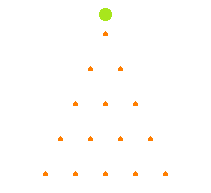
\includegraphics[width=2cm]{pins.png}
\captionof{figure}{Bumbiņa un tapiņu trīsstūris}
\label{fig:pins}
\end{center}

Aprēķiniet cik daudz dažādos ceļos bumbiņa var nonākt uz katras no tapām! 
Vai šeit ir kāds sakars ar uzdevuma \textit{[Trīsstūra formula]} rezultātu?

\end{problem}
%

%3
\begin{problem}
\textit{[Jebkurš skaitlis]} 
Vai Paskāla trīsstūris satur skaitli 2018?
\end{problem}
%

%4
\begin{problem}
\textit{[Mistiskās pakāpes]} 
Cik reizes $101.$ Paskāla trīsstūra rindas elementu summa pārsniedz $100.$ rindas elementu summu?
\end{problem}
%

%5
\begin{problem}
\textit{[Kombinatoriskie pierādījumi]} 
Pierādiet kombinatoriski:
\begin{enumerate}
\item $\binom{2n}{2}=2\binom{n}{2} + n^2$
\item $\binom{2n+2}{n+1}=\binom{2n}{n+1} + 2\binom{2n}{n} + \binom{2n}{n-1}$
\end{enumerate}
\end{problem}
%

%6
\begin{problem}
\textit{[Binomiālā teorēma]} 
Pierādiet \textit{Binomiālo teorēmu}:
$$
(x+y)^n = \binom{n}{0}x^n+\binom{n}{1}x^{n-1}y+\binom{n}{2}x^{n-2}y^2+ \dots + \binom{n}{n-1}xy^{n-1} +\binom{n}{n}y^n = \sum_{i=0}^{n}{\binom{n}{i}x^{n-i}y^{i}}
$$
\end{problem}
%

%7
\begin{problem}
\textit{[Dažas summas]} 
Aprēķiniet sekojošas summas:
\begin{enumerate}
\item $\binom{5}{0}+2\binom{5}{1}+2^2\binom{5}{2}+\dots+2^5\binom{5}{5}$
\item $\binom{n}{0}-\binom{n}{1}+\binom{n}{2}-\dots+(-1)^n\binom{n}{n}$
\item $\binom{n}{0}+\binom{n}{1}+\binom{n}{2}+\dots+\binom{n}{n}$
\end{enumerate}
\end{problem}
%

%9
\begin{problem}
\textit{[Sienāzīša problēma*]} 
Apskatīsim bezgalīgu rūtiņu lentu uz kuras pirmās rūtiņas sēž sienāzītis. Viņš var vienā lēcienā pārlekt vai nu par vienu, vai nu par divām rūtiņām pa labi. Cik veidos sienāzītis var nokļūt uz $n$-tās rūtiņas?

\end{problem}
%

%10
\begin{problem}
\textit{[Binārās virknes*]} 
Apskatīsim virknes garumā $n-1$, kuras sastāv tikai no cipariem $0$ un $1$, pie kam starp katriem diviem cipariem $1$ atrodas vismaz viens cipars $0$. Aprēķiniet šādu dažādo virkņu skaitu!

\end{problem}
%

%11
\begin{problem}
\textit{[Bumbiņu problēma*]} 
Mums ir $m$ identiskas baltas un $n$ identiskas melnas bumbiņas ($m>n$). Cik veidos var šīs bumbiņas izkārtot virknē tā, ka nevienā vietā blakus neatrodas divas melnas bumbiņas?

\end{problem}
%

%12
\begin{problem}
\textit{[Paskāla diagonāle]} 
Pierādiet vienādību $\binom{n}{0}+\binom{n-1}{1}+\binom{n-2}{2}+\dots =F_{n+1}$

\end{problem}
%
\end{document}
